\documentclass[aps,letterpaper,11pt]{revtex4}

\usepackage{graphicx}
\usepackage{float}
\usepackage{verbatim}
\usepackage{amsmath}
\usepackage{amssymb}

\newcommand{\labno}{9}
\newcommand{\labtitle}{Developing a New Amusement Park Ride for $Joy \hspace{1mm} Ride^{TM} \hspace{1mm} Inc.$}
\newcommand{\authorname}{Kevin Truong}
\newcommand{\professor}{Dr. Melanie Lutz}
\newcommand{\classno}{Physics 006}
\newcommand{\labpartners}{Sean Casey, Kevin Castillo, Dulce Payan, et al}
\newcommand{\submitdate}{April 25,2017}

\begin{document}

\begin{titlepage}
\begin{center}
\hspace{-136mm}\boxed{{\Large \textsc{Lab No. \labno}}}\\\vspace{30mm}
{\Large \textsc{\labtitle} \\ \vspace{4pt}}
\rule[13pt]{\textwidth}{1pt}\\ \vspace{150pt}
{\large By: \authorname \\ \vspace{10pt}}
Lab Partners: \labpartners \\
Instructor: \professor \vspace{10pt} \\
Solano Community College\\ \classno \\ \vspace{10pt}
\submitdate
\end{center}
\end{titlepage}

\section{Abstract}

This experiment examined the use of the work-energy theorem to calculate the displacement of an object traveling in a particular path. In this experiment, gravitational potential energy, kinetic energy, and work done by friction were considered in the work-energy equation. From the work-energy equations it was possible to solve for the final velocity that the car had when coming off the table. Using the kinematic equations in the x and y direction with the new knowledge of the initial velocity when it comes off the table, it was possible to solve for the distance in the x-direction that the car would travel. The distance that the box was placed away from the bottom of the table was 94.55 cm and this resulted in a successful landing of the car! 

\section{Introduction}

Analyzing an objects motion and its interaction with the environment relative to an origin could be determined by the work-energy theorem:

$$ W_{other} + E_1 = E_2$$

where all the energy in a system is conserved. Energy can be broken up into many things, in this experiment we will be analyzing Gravitational Potential Energy which is dependent on the objects mass, the gravitation on the object, and the distance relative to the origin and the source of the gravitation. We will also analyze Kinetic Energy which is described by an objects motion, Kinetic Energy is defined by an objects mass and velocity. $W_{other}$ is the work done by the environment, in this experiment the object is affected by friction on the race track therefore the Work done by friction will be considered. 

When analyzing Energy, it is important to understand different states that the object is in at particular points in time because this is how energy will answer important questions. 

Kinematics was again important in this experiment to analyzing the final "stretch" of the experiment when the toy car propels from the edge of the table towards the box, using the general kinematic equation:

$$ x = x_0 + v_0t + \frac{1}{2}at^2$$

The kinematic equation deal with vector quantities like velocity and acceleration, therefore it can be broken up into x and y directional kinematic equations. 

\section{Experimental Details}

Equipment for this experiment includes a toy car, meter stick, toy car's race track, tape, and box. The toy car acted as the roller coaster cart, and traversed the race track. The meter stick was used to obtain data and to make sure that certain things were the correct distance apart.  The toy car's race track was the medium that the toy car moved through on it's way to the box. The tape was used for measurements, to show how high or far the car traveled after being released. The box acted as the "vat" that the car would land in after falling from the table. 

The experiment explored what distance, X, the box needed to be placed away from the table, so that the toy car would fly into the box after barely making the loop when released from a height, $h_i$. It was important to take certain important things into account, for example it was important to take into account the little edge on the table that would needed to be acounted for when measuring from the bottom of the table to where the box would be placed. Also the track was not flush with the table, so it was necessary to measure the height from the table to the race track because the axis that was used was flush with the race track, not with the table. And it was important to take into account the thickness of the cart to obtain the most accurate center of mass of the toy car. 

\begin{center}
\underline{Diagram 1}\\
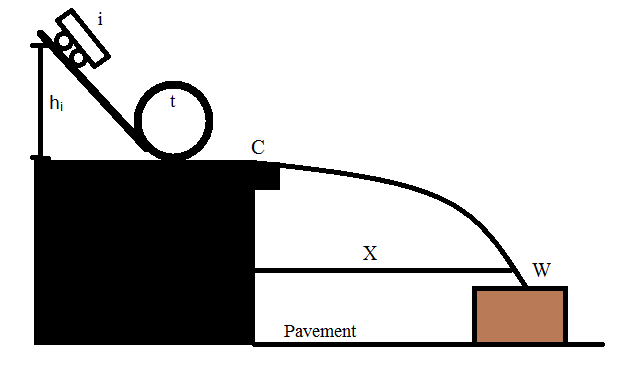
\includegraphics[width = 4in]{Setup.png}\\
\textit{Diagram 1: Setup to catch the Coaster}\\
\end{center}

\section{Results and Analysis}

\subsection{Finding the Height $h_i$}

When looking for $h_i$, we can use the work-energy methods. 

$$ mgh_i + W_{f}i \rightarrow t = \frac{1}{2}mv_t^2 + mg(2r-\bar{y})$$

The equation is using conservation of energy, analyzing the gravitational potential energy, kinetic energy, and work done by frictio to find nwhere W is the work done by friction when the cart travels from point i to point t on diagram 1, $h_i$ is the initial height that the cart needs to be placed to barely make the loop, $v_t$ is the tangential velocity of the car at point t, r is the radius of the loop, and $\bar{y}$ is the thickness of the car.   

looking at the equation directly above, known or directly measurable quantities would be gravity, the mass of the car, the radius of the loop, and the thickness of the car. Not directly measurable quantities would be the work done by friction, $h_i$, and the tangential velocity of the car at point t.

\subsubsection{Finding an Expression for $v_t$}

When finding the tangential velocity of the car at the top of the loop, we employed the condition that the car just barely makes it through the loop. For the car to barely make it through the loop, the force that the race track exerts onto the toy car will be zero. 

\begin{center}
\underline{Diagram 2}\\
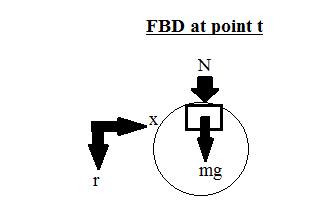
\includegraphics[width=4in]{FBDATT.png}\\
\textit{Diagram 2: Free body diagram at point t}
\end{center}

In this case when the toy car barely makes it through the loop, N is equal to zero. Therefore, when looking at the summation of forces in the r direction: 

$$ \sum_{}^{}F_r = ma_r$$

$$ mg = ma_r$$

In uniform circular motion the equation for radial acceleration is:

$$ a_r=\frac{v^2}{r}$$

however the radius from the center of the loop to the center of mass of the car is $(r-\bar{y})$

$$\therefore a_r = \frac{v^2}{r - \bar{y}}$$

And plugging this into the $a_r$ in our summation of forces in the r direction, simplifying the equation, and solving for $v_t$:

$$ v_t = \sqrt{g(r-\bar{y})}$$

now this equation can be subbed back into the initial equation found by looking at the conservation of energy:

$$ mgh_i + W_fi \rightarrow t = \frac{1}{2}m(g(r-\bar{y})) + mg(2r-\bar{y})$$

\subsubsection{Finding an Experssion for $W_fi \rightarrow t$}

To find the work done by friction from point i to point t, we must consider the work done by friction from point i to f in the following diagram:

\begin{center}
\underline{Diagram 3}\\
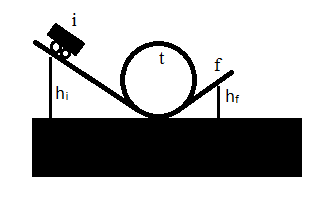
\includegraphics[width=4in]{WorkFromIToF.png}\\
\textit{Diagram 3: Altering the race track to create understand the work done by friction}
\end{center}

An assumption that was given during the experiment, is the work done by friction from point i to point t is about 60\% the work done by friction from point i to point f, where point f is the maximum distance that the car travels when released from a height, $h_i$. This assumption was reasonable because going from point i to point f is a farther distance than from point i to point t, so the work done by friction is greater when going from point i to point f. 

Since the car was released from rest, the kinetic energy of the car at point i is zero because the initial velocity when released is zero. At point f is the maximum distance that the car travels, so at point f the kinetic energy is zero because velocity at that point is zero. Looking at the work-Energy theorem again:

$$ W_fi \rightarrow f + mgh_i = mgh_f$$

Gravitational potential still exists because according to our axis, at the base of the race track, there is still some height away. 

When looking at the new work-energy equation directly above, the known or directly measurable quantities are m and g. The not directly measurable quantities are the work done by friction from point i to point f, $h_i$, and $h_f$.

It is difficult to solve for $h_i$ when $h_f$ is unkown, so we must consider another case. When the toy car is released from a greater, known, height $H_i$ which is the top of the race track and travels to a maximum distance and to a height relative to the table, $H_f$; which is also measurable when observing the maximum distnace traveled after being released from a height $H_i$.

\begin{center}
\underline{Diagram 4}\\
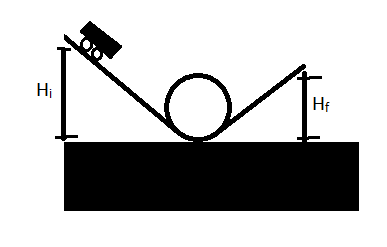
\includegraphics[width = 4in]{NEWCASE.png}\\
\textit{Diagram 4: New case considered to help find $h_i$}\\
\end{center}

Since the same race track was used and the only thing being altered is the height at which the toy car is being released, a ratio can found comparing the initial heights and final heights: 

$$ \frac{h_f}{h_i} = \frac{H_f}{H_i}$$

This assumption is reasonable because the same force of friction is working against the motion of the car and the same racetrack is used with the same angles between the incline/decline and the table. The only thing being altered is the heigh that the car is being released from, so it is safe to assume that the height being released will affect the final distance traveled, proportionally. Solving for $h_f$:

$$ h_f = (\frac{H_f}{H_i})h_i-+$$

Now substituting this into the work-energy equation found earlier and simplifying:

$$ W_f i \rightarrow f = mgh_i[\frac{H_f}{H_i}-1]$$

Since we said that it was reasonable to assume that $W_f i \rightarrow t = (0.6)W_f i \rightarrow f$:

$$ W_f i \rightarrow t = (0.6)(mgh_i[\frac{H_f}{H_i}-1])$$

Now plugging this into the equation solving for $h_i$ found earlier(The final equation in the "Finding an Expression for $v_t$" section), and simplifying the equation, the final equation for $h_i$ is:

$$ h_i = \frac{\frac{5}{2}r - \frac{3}{2}\bar{y}}{(0.6)\frac{H_f}{H_i} + 0.4}$$

Now $h_i$ has an equation with measurable quantities! The radius of the loop was measured with a meter stick and was found to be 12.85cm, the $\bar{y}$ or the thickness of the car was .775cm, the max initial height that the car was dropped from was 56.7cm, and the car traveled to a maximum final height of 32.66cm. Plugging these measured heights into the equation:

$$ h_i = \frac{\frac{5}{2}[12.85cm] - \frac{3}{2}[0.775cm]}{(0.6)\frac{[32.66cm]}{[56.7cm]} + 0.4} = \boxed{41.526cm}$$

$h_i$ was tested by looking at how the car traversed the loop when released from that height. We moved the car 3cm down from that height and saw that the car did not make the loop, and we moved the car 3cm up from that height and saw that the car easily traversed the loop. 

With the new calculated initial height, the car was released from rest and the new final height reached was $\approx 25.64cm$, the car was released five times and the average value was found to obtain a more accurate measurement. 

\subsection{Finding the Distance X}

Now that we found the the height that the car needs to be released to barely traverse the loop safely, we lower the end of the race track to the edge of the table and calculate the distance away from the bottom of the table that the box ("vat") needs to be placed, so the car can land in it. It's important to note that the car is in projectile motion after it leaves the edge of the table. Therefore it is important to know the initial velocity of the car as it leaves the edge of the table. Going back to diagram one, we can consider the work-energy theorem from point i to point C. 

At point i the car only has gravitational potential energy because it's being released from rest, at point c the car only has kinetic energy because the car is at the origin which was placed flush with the race track. However, there is the work done by friction as the car traverses the race track. The work-energy equation would look like:

$$ W_f i \rightarrow C + mgh_i = \frac{1}{2}mv_C^2$$

An important assumption that was made was that $W_f i \rightarrow f = W_f i \rightarrow C$. This assumption is dangerous because when the end of the track is inclined friction is equal to $\mu_kmgcos\theta$ where $\theta$ is the angle between the incline and the table, while friction when the track is leveled with the table is equal to $\mu_kmg$. However, the distance that the car travels is different in both cases; the distance that the car travels when going from point i to point C is a greater distance when going from point i to point f; so it could be possible that this change in distance will make up for the change in the friction force. 

Using the assumption in the experiment, the work done by friction when traveling from point i to point f can be substituted in for the work-energy equation just found:

$$ mgh_i + W_fi \rightarrow f = \frac{1}{2}mv_C^2$$

where $W_fi \rightarrow f$ was found earlier during part A of the experiment and it was:

$$W_fi \rightarrow f = mg(h_f - h_i)$$

Solving for $v_C$ and simplifying:

$$ v_C = \sqrt{2gh_f}$$

\begin{center}
\underline{Diagram 5}\\
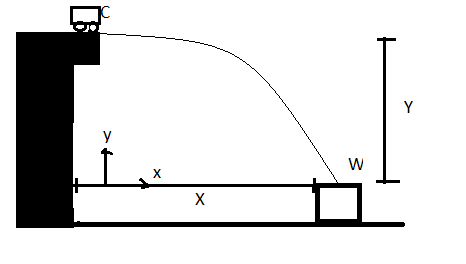
\includegraphics[width=4in]{ProjMotion.png}\\
\textit{Diagram 5: The projectile motion path}
\end{center}

Using the kinematic equations in the x-direction:

$$ x = x_0 +v_{0x}t + \frac{1}{2}a_xt^2$$

There is no acceleration in the x-direction,and the initial position in the x axis is at the origin therefore it's eqwual to zero as well.

$$ \Delta x = v_{0x}t$$

$v_{0x}$ was the initial velocity that the car comes off the table with, which is the equation for $v_C$.

$$ \therefore \Delta x = (\sqrt{2gh_f})t$$

Since the x and y components of the projectile motion will reach the point W at the exact same time, we can find the time it takes for the car to travel in the y direction to W and plug it into the equation for $\Delta x$ for t.

looking at the motion in the y-direction:

$$ y = y_0 + v_{0y}t + \frac{1}{2}a_yt^2$$

where the final y position will be zero because at point W it'll be level with the origin, $v_{0y}$ is also equal to zero because there was no vertical velocity once the car leaves the edge of the table; we can solve for t:

$$ t = \sqrt{\frac{2y_0}{g}}$$

Plugging this into the equation for $\Delta x$:

$$ \Delta x = (\sqrt{2gh_f})\sqrt{\frac{2y_0}{g}} = \boxed{2\sqrt{h_fy_0}}$$

Using a meter stick, $y_0$ was measured and found to be 82.8cm and $h_f$ was found earlier which was 25.64cm. However the table had a little "lip" at the edge of the table, so that needed to be accounted for; the "lip" had a length of 2.4cm. 

$$ \therefore \Delta x = 2\sqrt{(25.64cm)(82.8cm)} = 92.15cm + 2.4cm(length \hspace{1mm} of "lip") = \boxed{94.55cm}$$

After placing the box 94.55cm away from the bottom of the table, we placed the car at a height of $h_i$ + 3 cm and the car landed into the box on the first try!!

\section{Discussion} 

The experiment was a huge success because through meticulous calculation and measurements, we landed in the box on the first try! Some inaccuracies in the experiment may be due to the nature of the measurements, we measured distances using just a meterstick and eyeballed the measurements. The cart was given an additional 3 cm of height to deal with thses inaccuracies. The assumptions made were reasonable when it was thought thouroughly, and were necessary in solving the problem in this particular way.

\section{References}

\hspace{-6.5mm}
The Roller Splash Physics 06 Lab, Dr. Melanie Lutz\\



\end{document}
